\section{Review of Related Literature}
\label{sec:chapter_2}
\subsection{Homomorphic Cryptosystems}
A cryptosystem~\cite{bauer_cryptosystem_2005} consists of an encryption function and a decryption function, which operate on plaintexts, ciphertexts and keys. A \textit{plaintext}, is text that can be commonly understood within a larger group. Given a \textit{key} the encryption function maps a plaintext to some \textit{ciphertext}, which can only be understood by authorized parties. The decryption function similarly maps a ciphertext back to its corresponding plaintext, given an appropiate key. By sending data as ciphertext and only exposing the corresponding plaintexts to authorized parties who have access to the appropiate keys, secure data transmission can be achieved.

A \textit{homomorphic cryptosystem} allows operations to be performed on recovered plaintexts by performing corresponding operations on ciphertexts. This allows for secure computation by performing operations in the ciphertext domain. It is important to note that the operations in the plaintext space and ciphertext space need not be the same. A simple operation in the plaintext space may require a computationally intensive operation in the ciphertext space.

% \subsection{Partially Homomorphic Cryptosystems}
% A cryptosystem is called \textit{partially homomorphic} if it only admits limited types of operations on ciphtertexts. We present two partially homomorphic encryption (PHE) schemes: the Paillier cryptosystem and the DGK cryptosystem.  We then show how to use these PHE schemes for secure floating-point computation using two-party protocols. 

% big table to summarize Paillier and DGK
% \begin{table*}[ht]
% 	\caption{Summary of partially homomorphic cryptosystems}
% 	\label{tab:phe_summary}
%     \begin{tabular}{
%         p{\dimexpr 0.2\linewidth-2\tabcolsep}
%         p{\dimexpr 0.4\linewidth-2\tabcolsep}
%         p{\dimexpr 0.4\linewidth-2\tabcolsep}}
% 		\toprule
% 		 & Paillier & DGK\\
%         \midrule
%             Plaintext space &
%             $\mathbb{Z}_n$ &
%             $\mathbb{Z}_u$ 
%             \\
%             Ciphertext space &
%             $\mathbb{Z}_{n^2}$ &
%             $\mathbb{Z}^*_n$
%             \\
%             Key generation &
%             Define a function $L(x)$ as the largest integer $v$ greater than zero such that $x-1 \geq vn$.\newline
%             Choose two large primes $p$ and $q$, and set $n = pq, \lambda = \mathrm{lcm}(p-1,q-1)$.\newline
%             Select an integer $g$, $0\leq g \leq n^2$ such that $\mathrm{gcd}(L(g^\lambda \bmod n^2), n) = 1$\newline
%             The public key as $(g,n)$ and the private key $(p,q)$
%             &
%             Let $p,q$ be primes such that we can choose two primes $v_p$ and $v_q$ such that $v_p | (p-1)$ and $v_q | (q-1)$, and a small prime $u$ such that $u | (p-1)$ and $u | (q-1)$. \newline
%             Denote $n = pq$. \newline
%             Choose $g$ to be an integer of order $uv_pv_q$ and $h$ to be of order $v_pv_q$.\newline
%             The public key is $(n,g,h,u)$ and the private key is $(p,q,v_p,v_q)$.
%             \\
%             Encryption function &
%             $E(m) = g^m \cdot r^n \mod{n^2}$ &
%             $E(m) = g^m \cdot h^r \mod{n}$
%             \\
%             Decryption function &
%             $D(c) = L(c^\lambda \bmod n^2) \times (L(g^\lambda \bmod n^2))^{-1} \mod n$ &
%             Compute $c^{v_pv_q} \bmod n$. There is a one-to-one correspondence between this quantity and the plaintexts.
%             \\
% 	    \bottomrule
%     \end{tabular}
% \end{table*}
\subsection{Paillier and DGK Cryptosystems}
The Paillier cryptosystem \cite{stern_public-key_1999}, developed by Pascal Paillier, is a probabilistic encryption scheme which is based on the composite residuosity class problem. The scheme has several well--known homomorphic properties.
Table \ref{tab:paillier_summary} shows the key generation, encryption, and decryption procedures of the Paillier cryptosystem, which encrypts plaintexts in $\mathbb{Z}_n$ as ciphertexts in $\mathbb{Z}_{n^2}$.
\begin{table}[ht]
	\caption{The Paillier cryptosystem}
	\label{tab:paillier_summary}
    \begin{tabular}{
        p{\dimexpr 0.2\linewidth-2\tabcolsep}
        p{\dimexpr 0.8\linewidth-2\tabcolsep}}
		\toprule
		Step & Description\\
        \midrule
            Key\newline Generation &
            Let $L(x)$ be the largest integer $v$ greater than zero such that $x-1 \geq vn$.\newline
            Choose two large primes $p$ and $q$, and set $n = pq$, and $ \lambda = \mathrm{lcm}(p-1,q-1)$.\newline
            Select an integer $g$, $0\leq g \leq n^2$ such that $\mathrm{gcd}(L(g^\lambda \bmod n^2), n) = 1$\newline
            The public key as $(g,n)$ and the private key is $(p,q)$.
            \\
            Encryption &
            $E(m) = g^m \cdot r^n \mod{n^2}$ 
            \\
            Decryption &
            $D(c) = L(c^\lambda \bmod n^2) \times (L(g^\lambda \bmod n^2))^{-1} \mod n$ 
            \\
	    \bottomrule
    \end{tabular}
\end{table}
% The scheme allows for the encryption and decryption of integer messages, and is known to be additively homomorphic.
% We now state the encryption and decryption algorithms of the Paillier cryptosystem and its homomorphic properties.

% \paragraph{Key Generation}
% We first define a function $L(x)$ as the largest integer $v$ greater than zero such that $x-1 \geq vn$.
% We choose two large primes $p$ and $q$, and set $n = pq, \lambda = \mathrm{lcm}(p-1,q-1)$.
% Then we select an integer $g$, $0\leq g \leq n^2$ such that $\mathrm{gcd}(L(g^\lambda \bmod n^2), n) = 1$.
% We denote the public key as $(g,n)$ and the private key $(p,q)$.

% \paragraph{Encryption and Decryption}
% The encryption function to encrypt a plaintext $m \in \mathbb{Z}_n$ given a public key $(g,n)$ is defined as
% \begin{align*}
%   E(m) = g^m \cdot r^n \mod{n^2},
% \end{align*}
% where $r$ is a random non-negative integer less than $n^2$.

% The decryption function to decrypt a ciphertext $c \in \mathbb{Z}^\ast_{n^2}$ given a private key $(p,q)$ is defined as:
% \begin{align*}
%   D(c) = L(c^\lambda \bmod n^2) \times (L(g^\lambda \bmod n^2))^{-1} \mod n
% \end{align*}

% \paragraph{Homomorphic Properties of the Paillier Cryptosystem}
% The Paillier cryptosystem supports additive homomorphism as well as the multiplication of a plaintext scalar to an encrypted message. These homomorphic properties are used to add a plaintext scalar to a ciphertext, add two ciphertexts, and multiply a ciphertext by a plaintext scalar, respectively. They are defined as follows.

For all $m_1,m_2 \in \mathbb{Z}_n$ and $k\in \mathbb{N}$, the following homomorphic properties hold for the Paillier cryptosystem with public key $(g,n)$.
\begin{align*}
  D(E(m_1)g^k\bmod n^2) &=(m_1+k)\bmod n\\
  D(E(m_1)E(m_2)\bmod n^2) &=(m_1+m_2)\bmod n\\
  D(E(m_1)^k\bmod n^2) &= km_1\bmod n
\end{align*}

These homomorphic properties are used to add a plaintext to a ciphertext, add two ciphertexts, and multiply a ciphertext by a plaintext scalar, respectively.

The DGK cryptosystem was published by Damg{\aa}rd, Geisler, and Kr{\o}igaard in 2007 in an effort to create a secure integer comparison scheme \cite{pieprzyk_efficient_2007, cryptoeprint:2008:321} which is widely used in the literature \cite{veugen_improving_2012}.
 The details of the DGK cryptosystem may be found in Table \ref{tab:dgk_summary}. The DGK cryptosystem encrypts plaintexts in $\mathbb{Z}_u$ as ciphertexts in $\mathbb{Z}_n^\ast$, and has homomorphic properties similar to the Paillier cryptosystem.

\begin{table}[ht]
	\caption{The DGK cryptosystem}
	\label{tab:dgk_summary}
    \begin{tabular}{
        p{\dimexpr 0.2\linewidth-2\tabcolsep}
        p{\dimexpr 0.8\linewidth-2\tabcolsep}}
		\toprule
		Step & Description\\
        \midrule
            Key\newline Generation &
            Let $p,q$ be primes such that we can choose two primes $v_p$ and $v_q$ such that $v_p | (p-1)$ and $v_q | (q-1)$, and a small prime $u$ such that $u | (p-1)$ and $u | (q-1)$. \newline
            Denote $n = pq$. \newline
            Choose $g$ to be an integer of order $uv_pv_q$ and $h$ to be of order $v_pv_q$.\newline
            The public key is $(n,g,h,u)$ and the private key is $(p,q,v_p,v_q)$.
            \\
            Encryption &
            $E(m) = g^m \cdot h^r \mod{n}$
            \\
            Decryption &
            Compute $c^{v_pv_q} \bmod n$. There is a one-to-one correspondence between this quantity and the plaintexts, so the plaintext can be recovered using a lookup table.
            \\
	    \bottomrule
    \end{tabular}
\end{table}

For all $m_1,m_2 \in \mathbb{Z}_u$ and $k\in \mathbb{N}$, the following homomorphic properties hold for the DGK cryptosystem with public key $(n,g,h,u)$.
\begin{align*}
    D(E(m_1)g^k) &=(m_1+k)\bmod u\\
    D(E(m_1)E(m_2)) &=(m_1+m_2)\bmod u\\
    D(E(m_1)^k) &= km_1\bmod u
\end{align*}

As the multiplicative homomorphism was not presented in the original paper, we provide a short proof here.
\begin{theorem}
    In the DGK cryptosystem with public key $(n,g,h,u)$ and private key $(p,q,v_p,v_q)$, it holds that $D(E(m_1)^k) = km_1\bmod u$.
\end{theorem}
\begin{proof}
  Let $m \in \mathbb{Z}_u$ and $k\in \mathbb{N}$.
  We consider $E(m)^k = (g^m \cdot h^r \bmod{n})^k\bmod n$.
  \begin{align*}
    (g^m \cdot h^r \bmod{n})^k \bmod n
    &= (g^m \cdot h^r)^k \bmod{n}\\
    &= (g^m)^k \cdot (h^r)^k \bmod{n}\\
    &= g^{km} \cdot (h^{kr}) \bmod{n}
  \end{align*}
  Since $r$ is a random integer, $kr$ is also a random integer, Therefore, $g^{km} \cdot (h^{kr}) \bmod{n} = E(m)^k$ is a valid encryption of the message $km$.
\end{proof}

We have shown how the Paillier and DGK cryptosystems have similar homomorphic properties. In both cryptosystems, we are able to add a plaintext to a ciphertext, add two ciphertexts, and multiply a ciphertext by a plaintext scalar.
In order to use these cryptosystems in secure image processing, we require the two schemes to support the encryption and manipulation of floating-point (FP) numbers, which can be done by using an approach shown in~\cite{ziad_cryptoimg:_2016}. This approach represents FP numbers using an encrypted mantissa and an unencrypted exponent. This representation extends the addition and plaintext multiplication homomorphisms of the Paillier and DGK cryptosystems to floating-point numbers.

Table \ref{tab:flop_summary} describes protocols such as division~\cite{boukoros_lightweight_2017}, exponentiation~\cite{hutchison_privacy-preserving_2009}, and multiplication. These protocols, used in conjunction with the FP extension, allow for secure floating-point arithmetic~\cite{pcsc-paper}.

\begin{table}[ht]
	\caption{Two-party FP protocols}
	\label{tab:flop_summary}
    \begin{tabular}{
        p{\dimexpr 0.25\linewidth-2\tabcolsep}
        p{\dimexpr 0.75\linewidth-2\tabcolsep}}
		\toprule
		Operation & Protocol\\
        \midrule
            Division &
            The server selects a random number $r$ and sends $E(rx)$ and $E(ry)$ to the client, who can decrypt to obtain $rx$ and $ry$. The client then encrypts the quotient and sends $E(rx/ry) = E(x/y)$ to the server. 
            \\
            Exponentiation &
            The server selects a random number $r$ and computes $E\left(x+r\right)$. The server sends $E(x+r)$  to the client, who can decrypt to obtain $x+r$. The client then encrypts and sends $E((x+r)^2)$ to the server. The server then computes $E\left(\left(x+r\right)^2\right)E\left(-2rx + r^2\right) = E\left(x^2\right)$.
            \\
            Multiplication &
            The server obtains $E(x^2)$, $E(y^2)$, and $E((x+y)^2)$ using the exponentiation protocol. It can then compute $\frac{1}{2}E\left(\left(x+y\right)^2\right)E\left(x^2\right)^{-1}E\left(y^2\right)^{-1} = E\left(xy\right)$.\\
	    \bottomrule
    \end{tabular}
\end{table}
\subsection{The BGV Cryptosystem}
The BGV (Brakerski--Gentry--Vaikuntanathan) cryptosystem \cite{cryptoeprint:2011:277} is a fully homomorphic cryptosystem created based on the ring-learning with error problem. A \textit{fully homomorphic cryptosytem} allows aribitrary computation on encrypted data.
However, they are known to be significantly slower than partially homomorphic cryptosytems; improving the efficiency of fully homomorphic cryptosytems is an active area of research \cite{sen_homomorphic_2013}. 
The details regarding the construction of the BGV cryptosystem are beyond the scope of this paper. 

For this study, we will be using \textit{HELib}~\cite{garay_algorithms_2014}, an open-source library which implements the BGV cryptosystem with optimizations. \textit{HELib} supports arithmetic operations on integer ciphertexts and logical operations on binary ciphertexts. Evaluation of operations on 120 inputs in \textit{HELib} was performed in around 4 minutes, with an average of 2 seconds to process a single input~\cite{hutchison_fully_2010,cryptoeprint:2011:566}. The \textit{HELib} library has been adapted to Python using the Pyfhel library \cite{pyfhel_2018} maintained by Ibarrondo, Laurent (SAP) and Onen (EURECOM), and licensed under the GNU GPL v3 license.  
\subsection{CryptoImg}
A paper published in 2009 by Ziad, et al. implements privacy-preserving image processing using \textit{CryptoImg}, a library for the Open Source Computer Vision Library (OpenCV)~\cite{bradski_opencv_2000} which implements various homomorphic encryption and image processing routines using the Paillier homomorphic cryptosystem~\cite{ziad_cryptoimg:_2016}. The \textit{CryptoImg} library assumed a client-server model wherein a client requests image processing operations from a server. A client first encrypts a digital image and sends the image securely to a server, which then operates on the encrypted image without revealing its contents. Then the resulting image is sent back to the client, which decrypts the image to recover the desired output.
\begin{figure}[!ht]
    \centering
    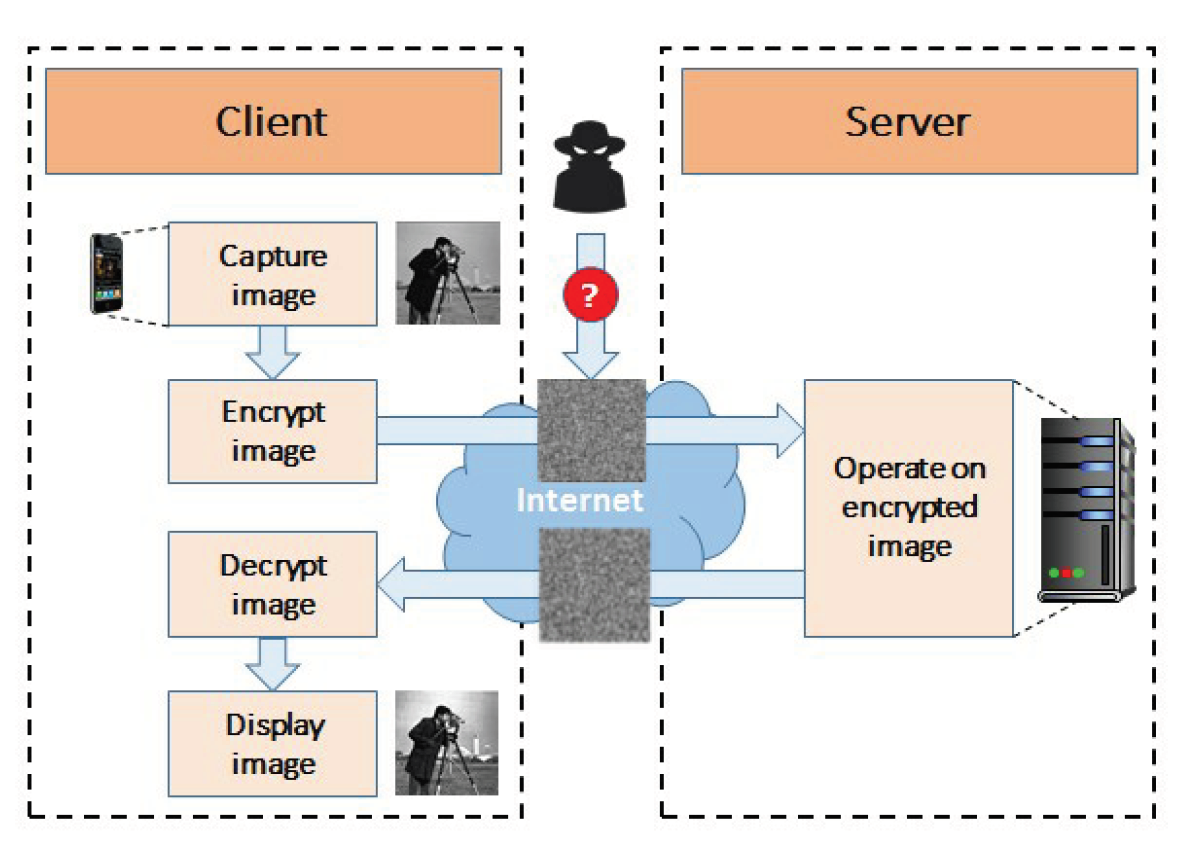
\includegraphics[width=0.4\textwidth]{figures/ClientServerModel.png}
    \caption{Client-server architecture used by \textit{CryptoImg} \cite{ziad_cryptoimg:_2016}}
    \label{fig:clientserver}
\end{figure}

The \textit{CryptoImg} library implemented the following image processing operations: image negation, brightness adjustment, spatial filters (for noise reduction, edge detection and sharpening), morphological operations, and histogram equalization.

% For image negation and spatial filters, the protocols specified by \textit{CryptoImg} allow all image processing operations to be performed on the server. However, due to limitations in the Paillier cryptosystem, the protocols presented for morphological operations and histogram equalization require both the client and the server to perform image processing calculations, although the server performs a significant portion of the processing.

Ziad, et al. also showed experimental results establishing the relatively slow performance of image operations under a homomorphic cryptosystem. For instance, while sharpening and applying a Sobel filter each take less than a second when applied to a $512\times 512$ plaintext image, when applied to an encrypted image, sharpening required at least 238.257 seconds, and applying the Sobel filter required at least 147.567 seconds \cite{ziad_cryptoimg:_2016}.


% We now discuss several limitations in the \textit{CryptoImg} study which we focus on for our research. First, the \textit{CryptoImg} library was limited in the image intensity transformations it implemented. We propose additional protocols to support more computationally intensive intensity transformations.
% Second, the \textit{CryptoImg} library only considered the Paillier cryptosystem. We consider testing the performance of other homomorphic cryptosystems, which differ in their processing time and supported operations.

% Convert to single table
\subsection{Image Intensity Transformations}
We represent a digital image $R$ as an $M \times N$ matrix of pixel intensity values, each value in the range $\left[0, L-1\right]$, for some positive integer $L$. We denote with $R(x,y)$ the entry at the $x$th row and $y$th column of a matrix $R$.
An intensity transformation on an image $R$ can be defined as a function $T$ which is applied to every pixel $r$ in $R$.
The \textit{CryptoImg} library implemented two types of linear intensity transformations: image negation and brightness control. An image negation transformation is defined as
\begin{equation}
    T\left(r\right) = L-1-r,
\end{equation}
which results in an image similar to a photographic negative~\cite{gonzalez_digital_2008}.
A brightness control transformation with parameter $v$ is defined as
\begin{equation}
    T\left(r,v\right) = r+v.
\end{equation}
The above transformations are linear in terms of the input $r$, and are thus simple to implement under a homomorphic cryptosystem.

In this study we extend the range of intensity transformations to non-linear transformations. Two common non-linear image transformations are the logarithm transformation and power-law transformation~\cite{gonzalez_digital_2008}.

The logarithm transformation is used to enhance dark pixels or increase the dark details of an image by mapping low intensity values to a wider range of values~\cite{gonzalez_digital_2008}. This has the general formula
\begin{equation}
    T\left(r\right) = c \log\left(1 + r\right)
\end{equation}
where $c$ is a constant.
The power-law transformation is a family of transformations that have the form
\begin{equation}
    T\left(r\right) = c r^{\gamma}
\end{equation}
where $c>0$ and $\gamma > 0$.
A power-law transformation can calibrate the operation of many image capture and output devices such as cameras, printers and displays in a process called \textit{gamma correction}.
% This ensures reproducibility and accuracy of images being displayed by digital output devices~\cite{gonzalez_digital_2008}.

To implement non-linear intensity transformations using addition and multiplication in a homomorphic system, it is necessary to approximate the logarithm and exponential functions, which may result in higher computational overhead. An applicable approximation for the logarithm may be found in \cite{pcsc-paper}. 
% In our software library implementation, we investigate methods required to approximate the logarithm and power functions. 
Non-linear intensity transformations such as the logarithm transformation have applications in intensity normalization \cite{oravec_illumination_2010}, which is used in some facial recognition algorithms to account for differences in lighting which make facial recognition difficult.

\subsection{Facial Detection and Recognition}

Since simple image operations mentioned earlier can be done within a homomorphic cryptosystem, these operations can be assembled together in order to do more complex operations. A prominent application of image processing that often uses complex image operations is \textit{facial recognition}.

Traditional facial recognition algorithms rely on detecting salient features in a face image. One of the popular facial recognition algorithms is \textit{eigenfaces}.
% Traditional facial recognition algorithms rely on detecting salient features in a face image. Two of the popular facial recognition algorithms are \textit{eigenfaces} and \textit{Haar cascades}.

\subsubsection{Eigenfaces}
Proposed by Matthew Turk and Alex Pentland, the eigenfaces method uses principal component analysis (PCA) in order to express an input image as a linear combination of eigenfaces \cite{turk_eigenfaces_1991}. An \textit{eigenface} is a principal component, or more simply an eigenvector that represents a certain variation between the face images which are taken from the initial training set. The number of resulting eigenfaces is equal to the number of face images in the training set.

% In the enrollment process, $M$ face images $\Theta_1, \ldots, \Theta_M$, each of size $p \times q$, are taken in to comprise the initial training set. The training images can be represented as vectors of length $N = pq$, where each row of an image is concatenated together.

% The average of the training images, denoted as $\Psi$, is
% \begin{equation}
% 	\Psi = \frac{1}{M} \sum_{i=1}^{M} \Theta_i
% \end{equation}

% The \textit{difference vectors} are then computed as $\Phi_i = \Theta_i - \Psi$. PCA is applied on the covariance matrix of the vectors
% \begin{equation}
% 	\mathbf{C} = \frac{1}{M} \sum_{i=1}^M \Phi_i \Phi_i^\top = \frac{1}{M} \mathbf{A}\mathbf{A}^\top,
% \end{equation}
% where $\mathbf{A}$ is an $N \times M$ matrix defined by $\left[\Theta_1 \quad \Theta_2 \quad \cdots \quad \Theta_M\right]$, in order to determine the orthonormal eigenvectors \cite{hutchison_privacy-preserving_2009}.

% Directly computing the covariance matrix and then applying PCA will become inefficient for large sizes of $\mathbf{A}$, since computing for $\mathbf{A}\mathbf{A}^\top$ results in an $N \times N$ matrix, which can get drastically large because it is dependent on the size of the image. On the other hand, computing for $\mathbf{A}^\top\mathbf{A}$ only results in an $M \times M$ matrix, which is much smaller than the previous one because it is just dependent on the number of face images in the training set. Now, we can apply PCA to $\mathbf{A}^\top\mathbf{A}$ along with some post-processing to obtain the eigenvectors \cite{hutchison_privacy-preserving_2009}.

% Instead of getting the eigendecomposition of the covariance matrix by explicitly computing the eigenvalues and eigenvectors of $\mathbf{C}$, we can also apply \textit{singular value decomposition} (SVD) on the matrix $\Phi^\top$. This is because SVD works through a divide-and-conquer method which results in greater numerical stability, while eigendecomposition simply uses the traditional QR factorization \cite{nakatsukasa_stable_2013, gu_divide-and-conquer_1995}. Upon applying SVD, we now get the eigenvectors $\mathbf{u}_1, \ldots, \mathbf{u}_M$ and their corresponding eigenvalues $\lambda_1, \ldots, \lambda_M$.

% We choose $K$ eigenvectors $\mathbf{u}_1, \ldots, \mathbf{u}_K$ such that it comprises a set associated with the $K$ largest eigenvalues, where $K$ is much smaller than $M$. This set is now the \textit{face space}. Then, the images $\Theta_1, \ldots, \Theta_K$ are projected onto the face space spanned by the eigenfaces to determine the weight vectors $\Omega_1, \ldots, \Omega_K$.

% To perform the recognition process, the algorithm projects the input image $\Gamma$ onto the face space, and then comparing the projected image $\bar{\Omega} = \mathbf{u}_i\left(\Gamma - \Psi\right)$ with each eigenface in the face space using a metric such as the Euclidean distance. Thus it is computed as $d_i = \left\lVert \Omega_i -\bar{\Omega} \right\rVert$ for all $i=1,\ldots,K$, where $\left\lVert \cdot \right\rVert$ denotes the Euclidean norm.

% Then, a match can be reported if the smallest possible distance is smaller than the given threshold value $T$.
% \newcommand{\argmin}{\mathop{\mathrm{arg\,min}}}
% \begin{equation}
% 	\text{ID} = \begin{cases}\argmin_i d_i & \text{if } \min_i d_i \le T \\\emptyset & \text {otherwise}\end{cases}
% \end{equation}


\subsection{Previous Implementations of Secure Facial Recognition}
Erkin, et al. \cite{hutchison_privacy-preserving_2009} devised a method to incorporate the use of homomorphic cryptosystems into the eigenfaces method. In their study, they proposed a two-party system where Alice holds an encrypted image $\left[\Gamma\right]$, while Bob maintains a database of $K$ eigenfaces $\mathbf{u}_1, \ldots, \mathbf{u}_K$, and feature vectors $\Omega_1, \ldots, \Omega_M$ in the clear.

\begin{figure}[h]
    \centering
    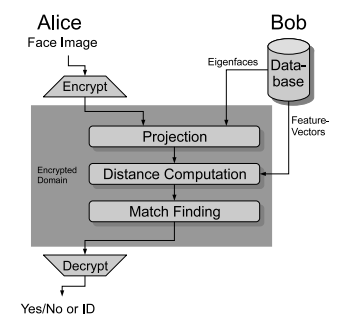
\includegraphics[width=0.4\textwidth]{figures/secure_eigenfaces.png}
    \caption{Diagram of the privacy-preserving facial recognition process \cite{hutchison_privacy-preserving_2009}}
\end{figure}

In order to ensure privacy, the steps in the eigenfaces algorithm, namely: projection, distance computation, and match finding, are done within the encrypted domain, i.e., using the operations in the Paillier cryptosystem.

Projection is similar to that of the original eigenfaces algorithm, except the operations are replaced with their respective operations in the cryptosystem. Distance computation in this version is somewhat different from the original eigenfaces method, in that it deals with the square of the Euclidean distance since the relative order of the distances is only important when comparing these during the match finding step \cite{hutchison_privacy-preserving_2009}.
\begin{align}
    d_i &= \left\lVert \Omega_i - \bar{\Omega} \right\rVert ^2 = \sum_{j=1}^{K} \left(\omega_{ij} - \bar{\omega}_j\right)^2 \\
        &= \underbrace{\sum_{j=1}^{K} \omega_{ij}^2}_{\mathcal{S}_1} + \underbrace{\sum_{j=1}^{K} \left(-2 \omega_{ij} \bar{\omega_j}\right)}_{\mathcal{S}_2} + \underbrace{\sum_{j=1}^{K} \bar{\omega}_{j}^2}_{\mathcal{S}_3}
\end{align}

Computing for the distances within Paillier would just be multiplying the encrypted sums together.
\begin{equation}
	\left[d_i\right] = \left[\mathcal{S}_1\right] \cdot \left[\mathcal{S}_2\right] \cdot \left[\mathcal{S}_3\right]
\end{equation}

The terms $\left[\mathcal{S}_1\right]$ and $\left[\mathcal{S}_2\right]$ can be easily computed by Bob, since he already knows both $\omega_i$ in the clear and $\left[\bar{\omega}_i\right]$ which is in encrypted form. Computing for $\left[\mathcal{S}_3\right]$ is trickier because Bob cannot compute for $\left[\bar{\omega}_i^2\right]$ because pairwise multiplication is not supported in Paillier, that is why Bob needs help from Alice to square a number through a protocol described below \cite{hutchison_privacy-preserving_2009}.

Before Bob sends $\left[\bar{\omega}_i\right]$ to Alice for squaring, he adds a random number $r_i$ to compute $\left[x_i\right] = \left[\bar{\omega}_i + r_i\right] = \left[\bar{\omega}_i\right] \cdot \left[r_i\right]$, where $r_i$ is obviously distinct for every $i$, then sends $\left[x_i\right]$ to Alice. She then decrypts it and computes $x_i^2$, and then computes $\mathcal{S}_3^\prime = \sum_{i=1}^{K} x_i^2$, after which she encrypts the sum and sends $\left[\mathcal{S}_3^\prime\right]$ to Bob. Now, he can compute for $\left[\mathcal{S}_3\right]$ as follows:
\begin{equation}
	\left[\mathcal{S}_3\right] = \left[\mathcal{S}_3^\prime\right] \cdot \prod_{j=1}^{K} \left(\left[\bar{\omega}_j\right]^{-2r_j} \cdot \left[-r_j^2\right]\right)
\end{equation}

The protocol for squaring a number as described earlier is a workaround for the limitations of Paillier or any other partially homomorphic cryptosystem that only supports addition and scalar multiplication.
% This can be possibly extended so that operations such as pairwise multiplication and exponentiation are also supported, provided that the protocol involves two parties.

The match-finding step is done by comparing the distances obtained from the previous step to a specified threshold $T$. If the minimum distance is smaller than $T$, then a match is found, and the encrypted identity of the match is returned to Alice \cite{hutchison_privacy-preserving_2009}. Getting the minimum among the encrypted distances would involve comparing two encrypted numbers, which Paillier does not support. Instead, the DGK cryptosystem \cite{pieprzyk_efficient_2007} is used for the comparison protocol.
